\documentclass{beamer}
\beamertemplatenavigationsymbolsempty
\usepackage{graphicx, tikz}


\begin{document}


\begin{frame}{Colouring Graphs}
\begin{columns}
\begin{column}{.5\textwidth}
\includegraphics[width=\textwidth]{Pictures/EnglishCounties.jpg}
\end{column}

\begin{column}{.5\textwidth}
\begin{block}{Started with 4 colour theorem:}
Any map can be coloured with four colours so that adjacent countries have different colours.
\begin{itemize}
\item Posed by Guthrie 1852
    \item Proved by Appel and Haken 1976
\end{itemize}    


\end{block}
\end{column}
\end{columns}
\begin{definition}The \emph{chromatic number} $\chi(G)$ of a graph $G$ is the least number of colours needed to colour the vertices so that adjacent vertices have different colours.
\end{definition}
\begin{theorem}[The four colour theorem]
A planar graph $G$ has $\chi(G)\leq 4$.
\end{theorem}
\end{frame}

\begin{frame}{First examples of chromatic number}
\begin{block}{The empty graph $E_n$}
The only graphs with $\chi(G)=1$ are the empty graphs $E_n$.
\end{block}
\begin{block}{The complete graph $K_n$}
The complete graph has $\chi(K_n)=n$
\end{block}

\begin{block}{Bipartite graphs}
A graph $G$ has $\chi(G)=2$ if and only if $G$ is bipartite.
\end{block}
\begin{block}{The wheel graph $W_n$}
$$\chi(W_n)=\begin{cases} 3 & n \text{ even} \\
4 & n \text{ odd}
\end{cases}$$
Why?
\end{block}

\end{frame}

\begin{frame}{How to find $\chi(G)$: sandwich it!}
Start by finding rough upper and lower bounds.

  \begin{block}{Upper bound: colour it}
If you can colour the vertices of $G$ with $k$ colours so that adjacent vertices don't share a vertex, then $\chi(G)\leq k$.
  \end{block}


  \begin{block}{Lower bound: often case by case}
    A few trivial tricks:
    \begin{itemize}
      \item If a vertex is adjacent to everything, as in $W_n$
      \item If $H$ is a subgraph of $G$, then $\chi(G)\geq \chi(H)$.
    \end{itemize}
    
    \end{block}
If lower bound isn't equal to upper bound, refine.  
\begin{block}{Finding the $\chi(G)$ is NP-hard}
So no beautiful answer.  But for small graphs not that bad.
  \end{block}

 \end{frame}

\begin{frame}{Example: find $\chi(G)$ for the graphs shown below}
  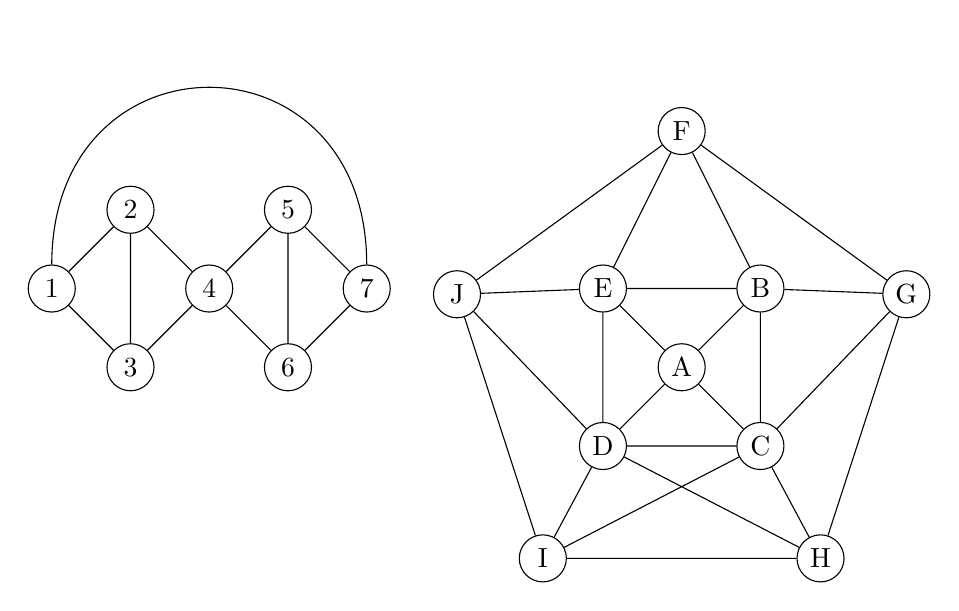
\begin{tikzpicture}
    \tikzstyle{vertex}=[circle, draw, minimum size=17pt, inner sep=0pt]
    \node[vertex] (1) at (0,1) {1};
    \node[vertex] (2) at (1,2) {2};
    \node[vertex] (3) at (1,0) {3};
    \node[vertex] (4) at (2,1) {4};
    \node[vertex] (5) at (3,2) {5};
    \node[vertex] (6) at (3,0) {6};
    \node[vertex] (7) at (4,1) {7};

    \draw (1)--(2)--(3)--(1);
    \draw (2)--(4)--(5)--(6)--(4)--(3);
    \draw (5)--(7)--(6);
    \draw (1) to[out=90, in=90, distance=3cm] (7);

    \begin{scope}[xshift=8cm]
      \node[vertex] (A) at (0,0) {A};
      \node[vertex] (B) at (1,1) {B};
      \node[vertex] (C) at (1,-1) {C};
      \node[vertex] (D) at (-1,-1) {D};
      \node[vertex] (E) at (-1,1) {E};
      \node[vertex] (F) at (90:3) {F};
      \node[vertex] (G) at (18:3) {G};
      \node[vertex] (H) at (-54:3) {H};
      \node[vertex] (I) at (234:3) {I};
      \node[vertex] (J) at (162:3) {J};

      \draw (B)--(C)--(A)--(B)--(E)--(A)--(D)--(C)--(G)--(B)--(F)--(G)--(H)--(I)--(J)--(D)--(I)--(C)--(H)--(D)--(E)--(J)--(F)--(E);




      

      \end{scope}
    
    \end{tikzpicture}


  
  \end{frame}


\begin{frame}{General upper bounds}
  \begin{definition}$\Delta(G)$ is the maximum degree of any vertex of $G$.
\end{definition}
    
\begin{lemma}
$$\chi(G)\leq \Delta(G)+1$$
\end{lemma}
\begin{proof}
Colour the vertices one by one in any order.
  \end{proof}
\begin{block}{The bound is tight, but for very few graphs:}
  \begin{itemize}
    \item $\chi(K_n)=n=\Delta(K_n)+1$
    \item For $n$ odd, $\chi(C_n)=3=\Delta(C_n)+1$
  \end{itemize}
  \begin{theorem}[Brooks]
If $G$ isn't a complete graph or an odd cycle, then $\chi(G)\leq \Delta(G)$.
    \end{theorem}

  \end{block}

  \end{frame}

\begin{frame}{A story problem for $\chi(G)$ -- not on exam this year}
  Suppose you have some things you want to separate into groups, but certain things can't be in the same group.  How many groups do you need?
  \begin{itemize}
  \item Group vacation, several cottages, some people don't get on
  \item Storing chemicals, some react dangerously with each other
    \end{itemize}
\begin{block}{Make a graph $G$ with:}
  \begin{itemize}
  \item Vertices are the things
  \item Edges mean the vertices can't be in the same group
  \end{itemize}
  The groups are the colours.
\end{block}
\begin{block}{$\chi(G)$ is the lowest feasible number of groups}
  \end{block}
  


  \end{frame}


\end{document}
